\documentclass{article}

\usepackage[utf8]{inputenc}
\usepackage{geometry}
\usepackage{graphicx}
\usepackage{titling}
\usepackage{fancyhdr}
\usepackage{cmbright}

\geometry{
	a4paper,
	total={170mm, 257mm},
	left=20mm,
	top=20mm
}


\title{Chapter 5: Vehicle 5 - Logic}
\author{Fharook Shaik}
\date{02 December 2024}

\fancypagestyle{fancy}{
	\fancyhf{}
	\fancyfoot[R]{
\includegraphics[width=3cm]{images/BTULogo_englisch_grau_2x.png}}
	\fancyfoot[L]{\thedate}
	\fancyhead[L]{13869 - Braitenberg Vehicle Praktium}
	\fancyhead[R]{\theauthor}
}

\pagestyle{fancy}

\makeatletter
\renewcommand{\maketitle}{
	\thispagestyle{fancy}
	\null
	\vskip 1em
	\begin{center}
		{\LARGE \@title \par}
	\end{center}
	\vskip 3em
}
\makeatother


\begin{document}

	\maketitle

	\noindent\begin{tabular}{@{}ll}
		Student & \theauthor\\
		Professor &  Dr. Cunningham, Douglas\\
		Matrikel-Nr.: & 5014962
		 
	\end{tabular}

	\section*{Summary}
	In Chapter 5 of \textit{Vehicles: Experoments in Synthetic Phsycology}, Valentino Braitenberg explored how basic mechanisms, when carefully designed, can produce systems that mimic reasoning, computation and memory. By focusing on threshold devices-simple components that act as switches-it demonstrates how clever arrangements of these basic elements can create vehicles capable of surprisingly complex and intelligent behaviours. The vehicles introduced in this chapter challenge the idea that intelligence requires intricate designs, showing intead of how complexity can emerge from simplicity.


    \subsection*{The Law of Uphill Analysis and Downhill Invention}
    The chapter introduces the \textit{law of uphill analysis and downhill invention}, which explains why designing a system is much easier than figuring out how it works just by observing its behaviour. When analysing a system from outside, people often assume it is more complicated than it really is. For example, Vehicle 4b appears to "think" before acting, but its behaviour is governed by a simple threshold device waiting for activation. This tendency to overestimate complexity demonstrates how even basic mechanisms can appear sophisticated when observed externally.

    This principle helps set the stage for understanding Vehicle 5, whise seemingsly advanced behaviours are created through strategic arrangement of simple components.

    
    \subsection*{Threshold Devices and their Role in Behaviour}
    Thresold devices are at the core of the vehicles logical capabilities. These devices activate only when the input signal surpasses a set threshold, making them ideal for decision making. They can also amplify or block signals, with \textit{inhibitory} connections counteracting activation from other sources. By linking threshold devices in various configurations such as one-to-one, one-to-many or many-to-one designers create systems capable if processing and responding to information.

    Small delays in activation and an additional layer of complexity, making the devices seem like they are \textit{deliberating} before acting. This flexibility allows for behaviours that appear logical, intentional, and even intelligent.

	\begin{figure}[h]
		\centering
		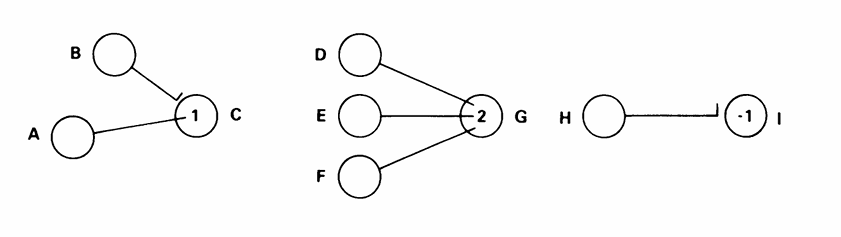
\includegraphics[scale=0.6]{images/figure_9.png}
		\caption{Thresold Devices and their interaction. L-Shaped fiber between B - C shows inhibition. A - C shows Activation. }
		\label{fig:vehicle-9}
	\end{figure}

    
    \subsection*{Vehicle 5: Logical Reasoning and Memory}
    Vehicle 5 demonstrates the power of threshold devices through its ability to perform logical operations, recognize patterns, and interact with its environment in advanced ways. For example, it can identify specific objects, such as an olive-green vehicle moving below 5 cm/sec, as if it "knows" and "names" certain entities.

    Vehicle 5 also interacts with numbers in interesting ways. It can count objects, associate with a specific number of vehicles (such as joining a group of four to make five), or avoid objects tied to "bad luck," such as multiples of seven. With enough threshold devices, Vehicle 5 can perform tasks like solving puzzles, playing chess, or even proving mathematical theorems. These advanced behaviors emerge from its simple design, highlighting how basic mechanisms can create the illusion of intelligence. 

    The chapter explores how Vehicle 5 develops memory. Memory arises from feedback loops between threshold devices, where one device keeps another activated, maintaining a signal that represents a past event. For example, if the vehicle detects red light, the loop stores this information, which can later trigger an action like ringing a bell. 

	\begin{figure}[h]
		\centering
		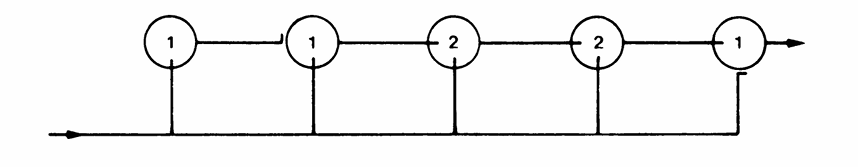
\includegraphics[scale=0.6]{images/figure_10a.png}
		\caption{Vehicle 10 Network that gives a signal when a burst of 3 pulses presents itself preceded and followed by a pause.}
		\label{fig:vehicle-10a}
	\end{figure}

    However, the internal memory of these systems is limited by the number of threshold devices. To overcome this limitation, vehicles can use their environment to store information. For instance, a vehicle might leave marks on the ground to record data it cannot store internally. It can later read these marks to continue calculations, effectively extending its computational capacity. This interaction between the vehicle and its surroundings demonstrates how simple systems can adapt and overcome internal constraints. 
	

    The chapter concludes by showing that networks of threshold devices can perform any task a modern computer can handle, including arithmetic, logic, and memory operations. These vehicles prove that intelligence does not require inherently complex designs. Instead, thoughtful arrangements of basic mechanisms can achieve behaviors that rival those of digital computers.  

    Vehicle 5's ability to play chess, solve puzzles, and handle numerical reasoning illustrates how simplicity can be transformed into universality. By leveraging threshold devices, even basic systems can replicate advanced reasoning and computation, challenging traditional ideas of complexity.


	\begin{figure}[h]
		\centering
		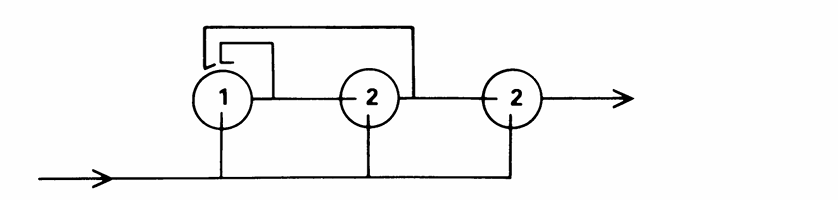
\includegraphics[scale=0.6]{images/figure_10b.png}
		\caption{Vehicle 10 Network of thresold devices that emits a pulse for every third pulse in a row in the input}
		\label{fig:vehicle-10b}
	\end{figure}

    \subsection*{Conclusion}
    Chapter 5 reveals how strategic design transforms simple mechanisms into systems capable of reasoning, memory, and computation. Vehicle 5 demonstrates that behaviors resembling intelligence can emerge from basic components when used creatively. This exploration challenges the assumption that complexity is necessary for intelligence, highlighting instead the power of simplicity.  

    By focusing on threshold devices and their applications, the chapter bridges the gap between simplicity and sophistication, showing how elementary systems can achieve extraordinary results.
	

\end{document}